

%% bare_conf.tex
%% V1.4b
%% 2015/08/26
%% by Michael Shell
%% See:
%% http://www.michaelshell.org/
%% for current contact information.
%%
%% This is a skeleton file demonstrating the use of IEEEtran.cls
%% (requires IEEEtran.cls version 1.8b or later) with an IEEE
%% conference paper.
%%
%% Support sites:
%% http://www.michaelshell.org/tex/ieeetran/
%% http://www.ctan.org/pkg/ieeetran
%% and
%% http://www.ieee.org/

%%*************************************************************************
%% Legal Notice:
%% This code is offered as-is without any warranty either expressed or
%% implied; without even the implied warranty of MERCHANTABILITY or
%% FITNESS FOR A PARTICULAR PURPOSE! 
%% User assumes all risk.
%% In no event shall the IEEE or any contributor to this code be liable for
%% any damages or losses, including, but not limited to, incidental,
%% consequential, or any other damages, resulting from the use or misuse
%% of any information contained here.
%%
%% All comments are the opinions of their respective authors and are not
%% necessarily endorsed by the IEEE.
%%
%% This work is distributed under the LaTeX Project Public License (LPPL)
%% ( http://www.latex-project.org/ ) version 1.3, and may be freely used,
%% distributed and modified. A copy of the LPPL, version 1.3, is included
%% in the base LaTeX documentation of all distributions of LaTeX released
%% 2003/12/01 or later.
%% Retain all contribution notices and credits.
%% ** Modified files should be clearly indicated as such, including  **
%% ** renaming them and changing author support contact information. **
%%*************************************************************************


% *** Authors should verify (and, if needed, correct) their LaTeX system  ***
% *** with the testflow diagnostic prior to trusting their LaTeX platform ***
% *** with production work. The IEEE's font choices and paper sizes can   ***
% *** trigger bugs that do not appear when using other class files.       ***                          ***
% The testflow support page is at:
% http://www.michaelshell.org/tex/testflow/



\documentclass[conference]{IEEEtran}
% Some Computer Society conferences also require the compsoc mode option,
% but others use the standard conference format.
%
% If IEEEtran.cls has not been installed into the LaTeX system files,
% manually specify the path to it like:
% \documentclass[conference]{../sty/IEEEtran}





% Some very useful LaTeX packages include:
% (uncomment the ones you want to load)


% *** MISC UTILITY PACKAGES ***
%
%\usepackage{ifpdf}
% Heiko Oberdiek's ifpdf.sty is very useful if you need conditional
% compilation based on whether the output is pdf or dvi.
% usage:
% \ifpdf
%   % pdf code
% \else
%   % dvi code
% \fi
% The latest version of ifpdf.sty can be obtained from:
% http://www.ctan.org/pkg/ifpdf
% Also, note that IEEEtran.cls V1.7 and later provides a builtin
% \ifCLASSINFOpdf conditional that works the same way.
% When switching from latex to pdflatex and vice-versa, the compiler may
% have to be run twice to clear warning/error messages.






% *** CITATION PACKAGES ***
%
%\usepackage{cite}
% cite.sty was written by Donald Arseneau
% V1.6 and later of IEEEtran pre-defines the format of the cite.sty package
% \cite{} output to follow that of the IEEE. Loading the cite package will
% result in citation numbers being automatically sorted and properly
% "compressed/ranged". e.g., [1], [9], [2], [7], [5], [6] without using
% cite.sty will become [1], [2], [5]--[7], [9] using cite.sty. cite.sty's
% \cite will automatically add leading space, if needed. Use cite.sty's
% noadjust option (cite.sty V3.8 and later) if you want to turn this off
% such as if a citation ever needs to be enclosed in parenthesis.
% cite.sty is already installed on most LaTeX systems. Be sure and use
% version 5.0 (2009-03-20) and later if using hyperref.sty.
% The latest version can be obtained at:
% http://www.ctan.org/pkg/cite
% The documentation is contained in the cite.sty file itself.






% *** GRAPHICS RELATED PACKAGES ***
%
\ifCLASSINFOpdf
  % \usepackage[pdftex]{graphicx}
  % declare the path(s) where your graphic files are
  % \graphicspath{{../pdf/}{../jpeg/}}
  % and their extensions so you won't have to specify these with
  % every instance of \includegraphics
  % \DeclareGraphicsExtensions{.pdf,.jpeg,.png}
\else
  % or other class option (dvipsone, dvipdf, if not using dvips). graphicx
  % will default to the driver specified in the system graphics.cfg if no
  % driver is specified.
  % \usepackage[dvips]{graphicx}
  % declare the path(s) where your graphic files are
  % \graphicspath{{../eps/}}
  % and their extensions so you won't have to specify these with
  % every instance of \includegraphics
  % \DeclareGraphicsExtensions{.eps}
\fi
% graphicx was written by David Carlisle and Sebastian Rahtz. It is
% required if you want graphics, photos, etc. graphicx.sty is already
% installed on most LaTeX systems. The latest version and documentation
% can be obtained at: 
% http://www.ctan.org/pkg/graphicx
% Another good source of documentation is "Using Imported Graphics in
% LaTeX2e" by Keith Reckdahl which can be found at:
% http://www.ctan.org/pkg/epslatex
%
% latex, and pdflatex in dvi mode, support graphics in encapsulated
% postscript (.eps) format. pdflatex in pdf mode supports graphics
% in .pdf, .jpeg, .png and .mps (metapost) formats. Users should ensure
% that all non-photo figures use a vector format (.eps, .pdf, .mps) and
% not a bitmapped formats (.jpeg, .png). The IEEE frowns on bitmapped formats
% which can result in "jaggedy"/blurry rendering of lines and letters as
% well as large increases in file sizes.
%
% You can find documentation about the pdfTeX application at:
% http://www.tug.org/applications/pdftex





% *** MATH PACKAGES ***
%
%\usepackage{amsmath}
% A popular package from the American Mathematical Society that provides
% many useful and powerful commands for dealing with mathematics.
%
% Note that the amsmath package sets \interdisplaylinepenalty to 10000
% thus preventing page breaks from occurring within multiline equations. Use:
%\interdisplaylinepenalty=2500
% after loading amsmath to restore such page breaks as IEEEtran.cls normally
% does. amsmath.sty is already installed on most LaTeX systems. The latest
% version and documentation can be obtained at:
% http://www.ctan.org/pkg/amsmath





% *** SPECIALIZED LIST PACKAGES ***
%
%\usepackage{algorithmic}
% algorithmic.sty was written by Peter Williams and Rogerio Brito.
% This package provides an algorithmic environment fo describing algorithms.
% You can use the algorithmic environment in-text or within a figure
% environment to provide for a floating algorithm. Do NOT use the algorithm
% floating environment provided by algorithm.sty (by the same authors) or
% algorithm2e.sty (by Christophe Fiorio) as the IEEE does not use dedicated
% algorithm float types and packages that provide these will not provide
% correct IEEE style captions. The latest version and documentation of
% algorithmic.sty can be obtained at:
% http://www.ctan.org/pkg/algorithms
% Also of interest may be the (relatively newer and more customizable)
% algorithmicx.sty package by Szasz Janos:
% http://www.ctan.org/pkg/algorithmicx




% *** ALIGNMENT PACKAGES ***
%
%\usepackage{array}
% Frank Mittelbach's and David Carlisle's array.sty patches and improves
% the standard LaTeX2e array and tabular environments to provide better
% appearance and additional user controls. As the default LaTeX2e table
% generation code is lacking to the point of almost being broken with
% respect to the quality of the end results, all users are strongly
% advised to use an enhanced (at the very least that provided by array.sty)
% set of table tools. array.sty is already installed on most systems. The
% latest version and documentation can be obtained at:
% http://www.ctan.org/pkg/array


% IEEEtran contains the IEEEeqnarray family of commands that can be used to
% generate multiline equations as well as matrices, tables, etc., of high
% quality.




% *** SUBFIGURE PACKAGES ***
%\ifCLASSOPTIONcompsoc
%  \usepackage[caption=false,font=normalsize,labelfont=sf,textfont=sf]{subfig}
%\else
%  \usepackage[caption=false,font=footnotesize]{subfig}
%\fi
% subfig.sty, written by Steven Douglas Cochran, is the modern replacement
% for subfigure.sty, the latter of which is no longer maintained and is
% incompatible with some LaTeX packages including fixltx2e. However,
% subfig.sty requires and automatically loads Axel Sommerfeldt's caption.sty
% which will override IEEEtran.cls' handling of captions and this will result
% in non-IEEE style figure/table captions. To prevent this problem, be sure
% and invoke subfig.sty's "caption=false" package option (available since
% subfig.sty version 1.3, 2005/06/28) as this is will preserve IEEEtran.cls
% handling of captions.
% Note that the Computer Society format requires a larger sans serif font
% than the serif footnote size font used in traditional IEEE formatting
% and thus the need to invoke different subfig.sty package options depending
% on whether compsoc mode has been enabled.
%
% The latest version and documentation of subfig.sty can be obtained at:
% http://www.ctan.org/pkg/subfig




% *** FLOAT PACKAGES ***
%
%\usepackage{fixltx2e}
% fixltx2e, the successor to the earlier fix2col.sty, was written by
% Frank Mittelbach and David Carlisle. This package corrects a few problems
% in the LaTeX2e kernel, the most notable of which is that in current
% LaTeX2e releases, the ordering of single and double column floats is not
% guaranteed to be preserved. Thus, an unpatched LaTeX2e can allow a
% single column figure to be placed prior to an earlier double column
% figure.
% Be aware that LaTeX2e kernels dated 2015 and later have fixltx2e.sty's
% corrections already built into the system in which case a warning will
% be issued if an attempt is made to load fixltx2e.sty as it is no longer
% needed.
% The latest version and documentation can be found at:
% http://www.ctan.org/pkg/fixltx2e


%\usepackage{stfloats}
% stfloats.sty was written by Sigitas Tolusis. This package gives LaTeX2e
% the ability to do double column floats at the bottom of the page as well
% as the top. (e.g., "\begin{figure*}[!b]" is not normally possible in
% LaTeX2e). It also provides a command:
%\fnbelowfloat
% to enable the placement of footnotes below bottom floats (the standard
% LaTeX2e kernel puts them above bottom floats). This is an invasive package
% which rewrites many portions of the LaTeX2e float routines. It may not work
% with other packages that modify the LaTeX2e float routines. The latest
% version and documentation can be obtained at:
% http://www.ctan.org/pkg/stfloats
% Do not use the stfloats baselinefloat ability as the IEEE does not allow
% \baselineskip to stretch. Authors submitting work to the IEEE should note
% that the IEEE rarely uses double column equations and that authors should try
% to avoid such use. Do not be tempted to use the cuted.sty or midfloat.sty
% packages (also by Sigitas Tolusis) as the IEEE does not format its papers in
% such ways.
% Do not attempt to use stfloats with fixltx2e as they are incompatible.
% Instead, use Morten Hogholm'a dblfloatfix which combines the features
% of both fixltx2e and stfloats:
%
% \usepackage{dblfloatfix}
% The latest version can be found at:
% http://www.ctan.org/pkg/dblfloatfix

\usepackage[]{todonotes}
\usepackage[outdir=./]{epstopdf}
\usepackage[ruled]{algorithm2e}
\usepackage{amsmath}

% *** PDF, URL AND HYPERLINK PACKAGES ***
%
%\usepackage{url}
% url.sty was written by Donald Arseneau. It provides better support for
% handling and breaking URLs. url.sty is already installed on most LaTeX
% systems. The latest version and documentation can be obtained at:
% http://www.ctan.org/pkg/url
% Basically, \url{my_url_here}.




% *** Do not adjust lengths that control margins, column widths, etc. ***
% *** Do not use packages that alter fonts (such as pslatex).         ***
% There should be no need to do such things with IEEEtran.cls V1.6 and later.
% (Unless specifically asked to do so by the journal or conference you plan
% to submit to, of course. )


% correct bad hyphenation here
\hyphenation{op-tical net-works semi-conduc-tor}


\begin{document}
%
% paper title
% Titles are generally capitalized except for words such as a, an, and, as,
% at, but, by, for, in, nor, of, on, or, the, to and up, which are usually
% not capitalized unless they are the first or last word of the title.
% Linebreaks \\ can be used within to get better formatting as desired.
% Do not put math or special symbols in the title.

\title{Parallel Standard Particle Swarm Optimization}


% author names and affiliations
% use a multiple column layout for up to three different
% affiliations
\author{Gian M. Fritsche}

% conference papers do not typically use \thanks and this command
% is locked out in conference mode. If really needed, such as for
% the acknowledgment of grants, issue a \IEEEoverridecommandlockouts
% after \documentclass

% for over three affiliations, or if they all won't fit within the width
% of the page, use this alternative format:
% 
%\author{\IEEEauthorblockN{Michael Shell\IEEEauthorrefmark{1},
%Homer Simpson\IEEEauthorrefmark{2},
%James Kirk\IEEEauthorrefmark{3}, 
%Montgomery Scott\IEEEauthorrefmark{3} and
%Eldon Tyrell\IEEEauthorrefmark{4}}
%\IEEEauthorblockA{\IEEEauthorrefmark{1}School of Electrical and Computer Engineering\\
%Georgia Institute of Technology,
%Atlanta, Georgia 30332--0250\\ Email: see http://www.michaelshell.org/contact.html}
%\IEEEauthorblockA{\IEEEauthorrefmark{2}Twentieth Century Fox, Springfield, USA\\
%Email: homer@thesimpsons.com}
%\IEEEauthorblockA{\IEEEauthorrefmark{3}Starfleet Academy, San Francisco, California 96678-2391\\
%Telephone: (800) 555--1212, Fax: (888) 555--1212}
%\IEEEauthorblockA{\IEEEauthorrefmark{4}Tyrell Inc., 123 Replicant Street, Los Angeles, California 90210--4321}}




% use for special paper notices
%\IEEEspecialpapernotice{(Invited Paper)}




% make the title area
\maketitle

% As a general rule, do not put math, special symbols or citations
% in the abstract
% \begin{abstract}
% The abstract goes here.
% \end{abstract}

% no keywords




% For peer review papers, you can put extra information on the cover
% page as needed:
% \ifCLASSOPTIONpeerreview
% \begin{center} \bfseries EDICS Category: 3-BBND \end{center}
% \fi
%
% For peerreview papers, this IEEEtran command inserts a page break and
% creates the second title. It will be ignored for other modes.
\IEEEpeerreviewmaketitle



% \title{Parallel Standard Particle Swarm Optimization}
% \author{Gian M. Fritsche}
% \date{\today}

% \begin{document}
%     \maketitle


    \section{Introduction}

    The Particle Swarm Optimization~\cite{PSO95} is a meta-heuristic based on the behavior of bird flocks. Every iteration, each particle moves in the search space based on three components:

    \begin{itemize}
        \item {\em Social:} This component contributes for the exploitation of the algorithm.
        It guides the search towards the best solutions found by the swarm.
        \item {\em Individual:} The individual component guides the particle to the best region that the particle has found.
        \item {\em Inertia:} The inertia component increase the exploration of the algorithm. It is responsible for keeping the particle moving towards a previous direction and avoid abrupt changes of direction.
    \end{itemize}

    The position of one particle is a set of variable values, {\em i.e.} a solution for an optimization problem. Then, the algorithms evaluate the solution, and a fitness value is associated. Based on the fitness value the Social and Individual components are updated.
    Moreover, these components are used to compute the next position of the particle (another solution for the problem).

    Since its first publication, the PSO had proposed several adaptations and improvements.
    In 2006 it was created the first version of a Standard Particle Swarm Optimization~\cite{SPSO}. The SPSO was not proposed to be the best PSO available, but establish a common benchmark as a baseline to assess the PSO variants in the literature.

    \subsection {Standard Particle Swarm optimization}

    Since its first publication (2006), there is three versions of SPSO: 2006, 2007 and 2011.
    In the latest version the description is given as follow (and showed in Algorithm~\ref{alg:spso2011}):
    The first population (set of solutions) is initialized randomly in the search space. Then, the algorithms initialize the velocity also randomly. The suggested population size is $40$. The neighborhood topology used to update the social component is the Adaptive Random Topology (ART).
    In the ART each particle informs its current fitness to $K$ neighbors. If the fitness is better than the previous social best information of the neighbor the social best (fitness and position) is updated. A direct graph represents the neighborhood, where each particle informs its quality to (at most) $K$ neighbors. The graph is generated randomly initially and every time that the best global fitness is not improved.

    In the previous versions of PSO, the velocity was updated dimension by dimension.
    However, in SPSO2011 the velocity is updated in a geometrical way,  that does not depend on the system of coordinates.

    \begin{algorithm}[!htb]
        \KwResult{The best solution and its fitness}
        
        create adaptive random neighbourhood\;

        \ForEach{particle $ i \in swarm$}{
            initialize particles' position ($\vec{X_i}$) and velocity ($\vec{V_i}$)\;
            evaluate particle ($f(\vec{X_i})$)\;
            initialize personal best ($\vec{P_i}$) and neighbour best ($\vec{G_i}$)\;
            update global best fitness ($best\_fitness=\min(f(\vec{X_i}), best\_fitness)$)\;
        }
        number of iterations ($T$) = 1\;
        \While{$T < MAX\_IT$  }{
            $previous\_best\_fitness = best\_fitness$\;
            \ForEach{particle $ i \in swarm$}{
                update particle's velocity ($\vec{V_i}$)\;
                update particle's position ($\vec{X_i}$)\;
                evaluate particle ($f(\vec{X_i})$)\;
                \If{ $f(\vec{X_i}) < f(\vec{P_i})$ }{
                    $\vec{P_i} = \vec{X_i}$\;
                }
                update neighbour best ($\vec{G_i}$)\;
                update global best fitness ($best\_fitness=\min(f(\vec{X_i}), best\_fitness)$)\;
            }
            \If{$previous\_best\_fitness \le best\_fitness$}{
                create adaptive random neighbourhood\;
            }

            $T=T+1$
        }
        \ForEach{particle $ i \in swarm$}{
            \If{$f(\vec{X_i}) == best\_fitness$}{
                $best\_solution = \vec{X_i}$\; 
            }
        }
        
        \caption{Standard Particle Swarm Optimization 2011}
        \label{alg:spso2011}
    \end{algorithm}

    \section{Parallel SPSO-2011}

    \subsection{Related works}

    In the literature, it is possible to find different proposals of Parallel PSOs.
    One of the most recent is the GPU-based Asynchronous Particle Swarm Optimization~\cite{GPUPSO}.
    That implements a simple ring topology.
    In~\cite{ReviewGPUPSO}, it is presented a review of Particle Swarm Optimization on GPU.
    The paper presents 28 references of PSO on GPU including multi-objective versions and variations of PSO from 2009 to 2014.
    One of the papers from the review implements the Standard Particle Swarm Optimization 2007 using GPU~\cite{GPUSPSO2007}. The GPU version was 11 times faster than the CPU, mainly with a large population and high dimensional problems.

    \subsection{Proposal}

    In this work, we use the SPSO2011, which uses the Adaptive Random Neighborhood topology.  
    During the literature review, it was not found any other implementation of the SPSO2011 using GPU.
    The parallel implementation associates each particle with one thread (Algorithm~\ref{alg:pspso2011}).
    In this way, all \texttt{{\bf foreach} particle $ i \in swarm$ } were removed and executed in parallel based on the thread id inside the block ($threadIdx.x$ or $tid$).
    In the create adaptive random neighborhood method each particle selects up to $K$ neighbors. Then the particle updates its position and velocity; the position is evaluated using the fitness function, and the personal best is updated.
    Then, to update the neighbor best information, the particle search on the adjacency matrix of the neighborhood for all its neighbors and compares to itself.
    The best global fitness is computed using atomic operations. The $atomicMin(a, b)$ was implemented based on the CUDA $atomicCAS$, which realizes a compare and swap operation.
    Before entering the main loop, the implementation applies a thread synchronization.

    The first particle copies the best fitness for later comparison.
    Inside the main loop, the particle (thread) updates its velocity, position, and fitness.
    The personal best information is updated.
    Before setting the neighbor best information a synchronization is necessary because the threads must compare its fitness to the updated value of its neighbors.
    Then, the neighbor best information is updated. Also, the best fitness is updated using the $atomicMin$ function.
    After the best fitness update, it is applied another \texttt{\_\_syncthreads()}. To wait for all threads update the best fitness before using its value.
    If the best fitness is not improved, then the new neighborhood matrix is generated.
    After $T$ iterations the solution with fitness equals to the best fitness is the output of the algorithm.

    \begin{algorithm}[!htb]
        \KwResult{The best solution and its fitness}
        
        $tid = threadIdx.x\;$

        create adaptive random neighbourhood\;
        \_\_syncthreads()\;

        initialize particles' position ($\vec{X_{tid}}$) and velocity ($\vec{V_{tid}}$)\;
        evaluate particle ($f(\vec{X_{tid}})$)\;
        initialize personal best ($\vec{P_{tid}}$) and neighbour best ($\vec{G_{tid}}$)\;
        \tcc{the update global best uses atomicMin operation}
        update global best fitness ($best\_fitness=\min(f(\vec{X_{tid}}), best\_fitness)$)\;
        \_\_syncthreads()\;
        number of iterations ($T$) = 1\;
        \While{$T < MAX\_IT$  }{
            \If{$tid == 0$}{
                $previous\_best\_fitness = best\_fitness$\;
            }
            
            update particle's velocity ($\vec{V_{tid}}$)\;
            update particle's position ($\vec{X_{tid}}$)\;
            evaluate particle ($f(\vec{X_{tid}})$)\;
            \If{ $f(\vec{X_{tid}}) < f(\vec{P_{tid}})$ }{
                $\vec{P_{tid}} = \vec{X_{tid}}$\;
            }
            \_\_syncthreads()\;
            update neighbour best ($\vec{G_{tid}}$)\;
            \tcc{the update global best uses atomicMin operation}
            update global best fitness ($best\_fitness=\min(f(\vec{X_{tid}}), best\_fitness)$)\;
            \_\_syncthreads()\;
            
            \If{$previous\_best\_fitness \le best\_fitness$}{
                create adaptive random neighbourhood\;
            }

            $T=T+1$
        }
        
        \If{$f(\vec{X_{tid}}) == best\_fitness$}{
            $best\_solution = \vec{X_{tid}}$\; 
        }
        
        \caption{Parallel Standard Particle Swarm Optimization 2011}
        \label{alg:pspso2011}
    \end{algorithm}

    In the first implemented version it was not used shared memory, but in a second implementation it was used and the execution time was improved.
    Another item important to highlight is the two \texttt{\_\_syncthreads()} inside the loop.
    The use of \texttt{\_\_syncthreads()} generally slow down the execution of a CUDA program.
    % However, in this implementation we did not have this problem due to the block size equals to warp size.
    % Since the threads in the same warp execute in true (hardware) parallelism, there is no situation where threads need to sync with others on the same block.

    The first experiments were executed using only one block. However, the experiments run the SPSO several times; those executions can be run in parallel, using different and independent blocks. In the experiments using only one block, the CPU implementation had a better execution time. However, when using multi executions at once, the GPU implementation achieved a better execution time.
    Those first experiments were executed using a simple function called Sphere.
    Then it was evaluated the scalability of the implementations increasing the population size. The population size defines the number of threads per block. For those experiments, it was used the Schaffer function.
    The next section details the experiments and results.

    \section{Experiments and Results}

    The first experiment was used to validate the equivalence regarding the quality of the GPU and CPU implementation. Both implementations showed similar convergence along the execution.

    For this first experiments it was used $T=3125$ iterations, $32$ particles, $D=10$ decision variables, $K=3$, and the Sphere function for fitness evaluation (this function is presented in Figure~\ref{fig:sphere}).  We executed $51$ independent runs. Those parameters were based on~\cite{SPSOCEC}. Moreover, the Sphere function is a simple optimization function present on the COCO (Comparing Continuous Optimisers) benchmark~\footnote{http://coco.gforge.inria.fr/}. The Sphere function is a minimization problem: 

    \begin{equation}
        f(x_1 \cdots x_n) = \sum_{i=1}^n x_i^2
    \end{equation}

    \begin{equation}
            -100.0 \leq x_i \leq 100.0
    \end{equation}

    \begin{equation}
       \text{minimum at }f(0, \cdots, 0) = 0
    \end{equation}

     \begin{figure}[!htb]
        \centering
        \includegraphics[width=\columnwidth]{../img/sphere.png}
        \caption{Sphere --- Two dimensional view}
        \label{fig:sphere}
    \end{figure}


    The Table~\ref{tbl:gpuinfo} presents the information about the used GPU.
    Besides, the Table~\ref{tbl:cpuinfo} presents the CPU information.

    \begin{table}[!htb]
        \centering
        \caption{GPU information}
        \label{tbl:gpuinfo}
        \begin{tabular}{|l|l|}
            \hline
            \multicolumn{2}{|c|}{\textbf{--- General Information for device 0 ---}} \\ \hline
            \textbf{Name}                          & GeForce GTX 680                \\ \hline
            \textbf{Compute capability}            & 3.0                            \\ \hline
            \textbf{Clock rate}                    & 1058500                        \\ \hline
            \textbf{Device copy overlap}           & Enabled                        \\ \hline
            \textbf{Kernel execution timeout}      & Disabled                       \\ \hline
            \multicolumn{2}{|c|}{\textbf{--- Memory Information for device 0 ---}}  \\ \hline
            \textbf{Total global mem}              & 2095382528                     \\ \hline
            \textbf{Total constant Mem}            & 65536                          \\ \hline
            \textbf{Max mem pitch}                 & 2147483647                     \\ \hline
            \textbf{Texture Alignment}             & 512                            \\ \hline
            \multicolumn{2}{|c|}{\textbf{--- MP Information for device 0 ---}}      \\ \hline
            \textbf{Multiprocessor count}          & 8                              \\ \hline
            \textbf{Shared mem per mp}             & 49152                          \\ \hline
            \textbf{Registers per mp}              & 65536                          \\ \hline
            \textbf{Threads in warp}               & 32                             \\ \hline
            \textbf{Max threads per block}         & 1024                           \\ \hline
            \textbf{Max thread dimensions}         & (1024, 1024, 64)               \\ \hline
            \textbf{Max grid dimensions}           & (2147483647, 65535, 65535)     \\ \hline
        \end{tabular}
    \end{table}

    \begin{table}[!htb]
        \centering
        \caption{CPU information}
        \label{tbl:cpuinfo}
        \begin{tabular}{|l|l|}
            \hline
            \textbf{vendor\_id} & GenuineIntel                             \\ \hline
            \textbf{cpu family} & 6                                        \\ \hline
            \textbf{model}      & 63                                       \\ \hline
            \textbf{model name} & Intel(R) Core(TM) i7-5930K CPU @ 3.50GHz \\ \hline
            \textbf{stepping}   & 2                                        \\ \hline
            \textbf{microcode}  & 0x36                                     \\ \hline
            \textbf{cpu MHz}    & 3599.941                                 \\ \hline
            \textbf{cache size} & 15360 KB                                 \\ \hline
        \end{tabular}
    \end{table}

    In the Figure~\ref{fig:semilogy_convergence} it is presented the average convergence of the algorithms (GPU and CPU) during the iterations. Where it is possible to observe similar behavior because they implement the same algorithm.
    As increasing the number of iteration better is the quality of the solutions. 
    That indicates that the implementations of GPU and CPU are equivalent in terms of solution quality.

    % \begin{figure}[!htb]
    %     \centering
    %     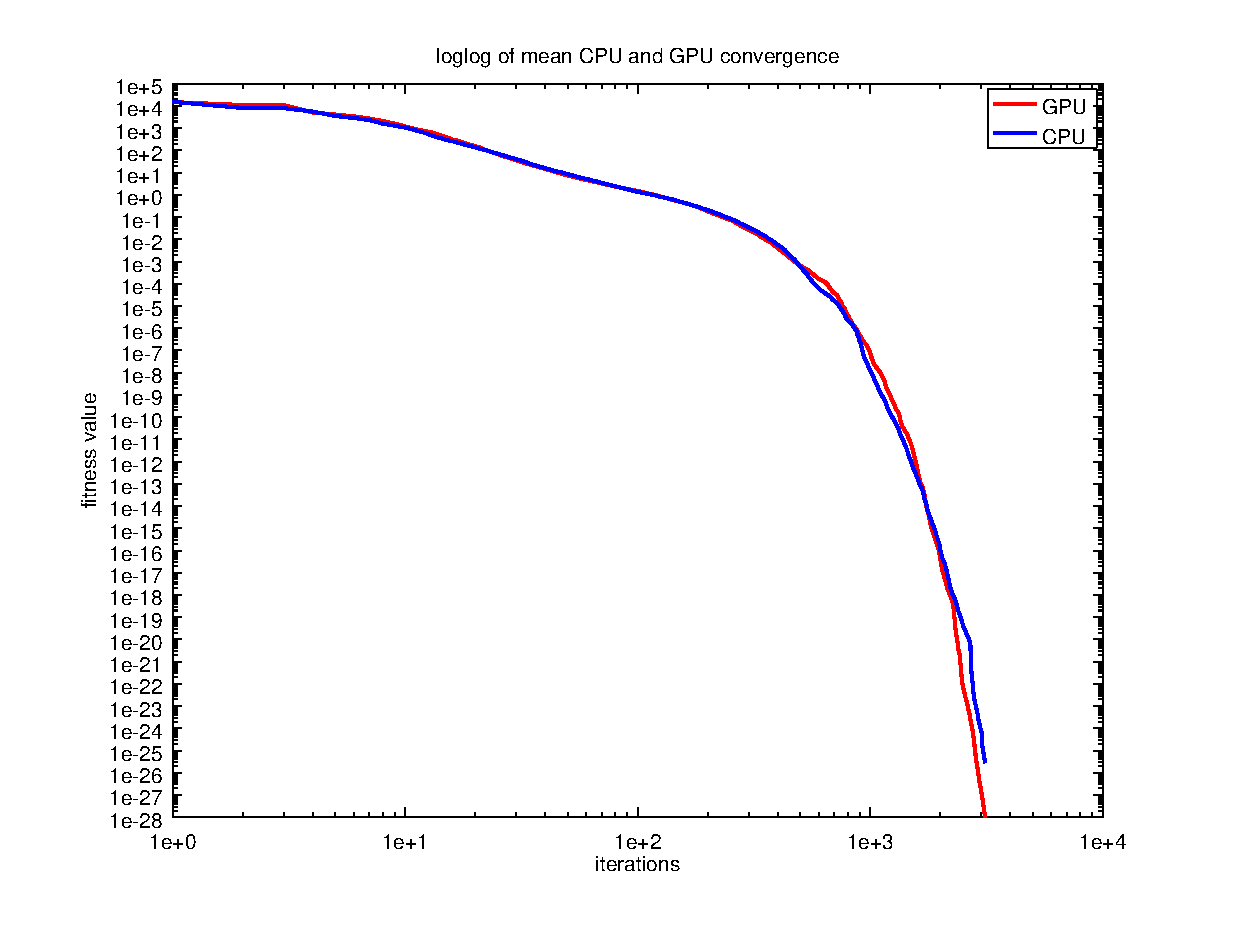
\includegraphics[width=\columnwidth]{../img/loglog_convergence.eps}
    %     \caption{loglog of the average quality of the solutions found by the implemented algorithms during the $3125$ iterations. As much more iterations, better is the quality of the solutions. Both CPU and GPU behaves similarly, as they implement the same algorithm}
    %     % \caption{loglog of mean CPU and GPU convergence}
    %     \label{fig:loglog_convergence}
    % \end{figure}

    \begin{figure}[!htb]
        \centering
        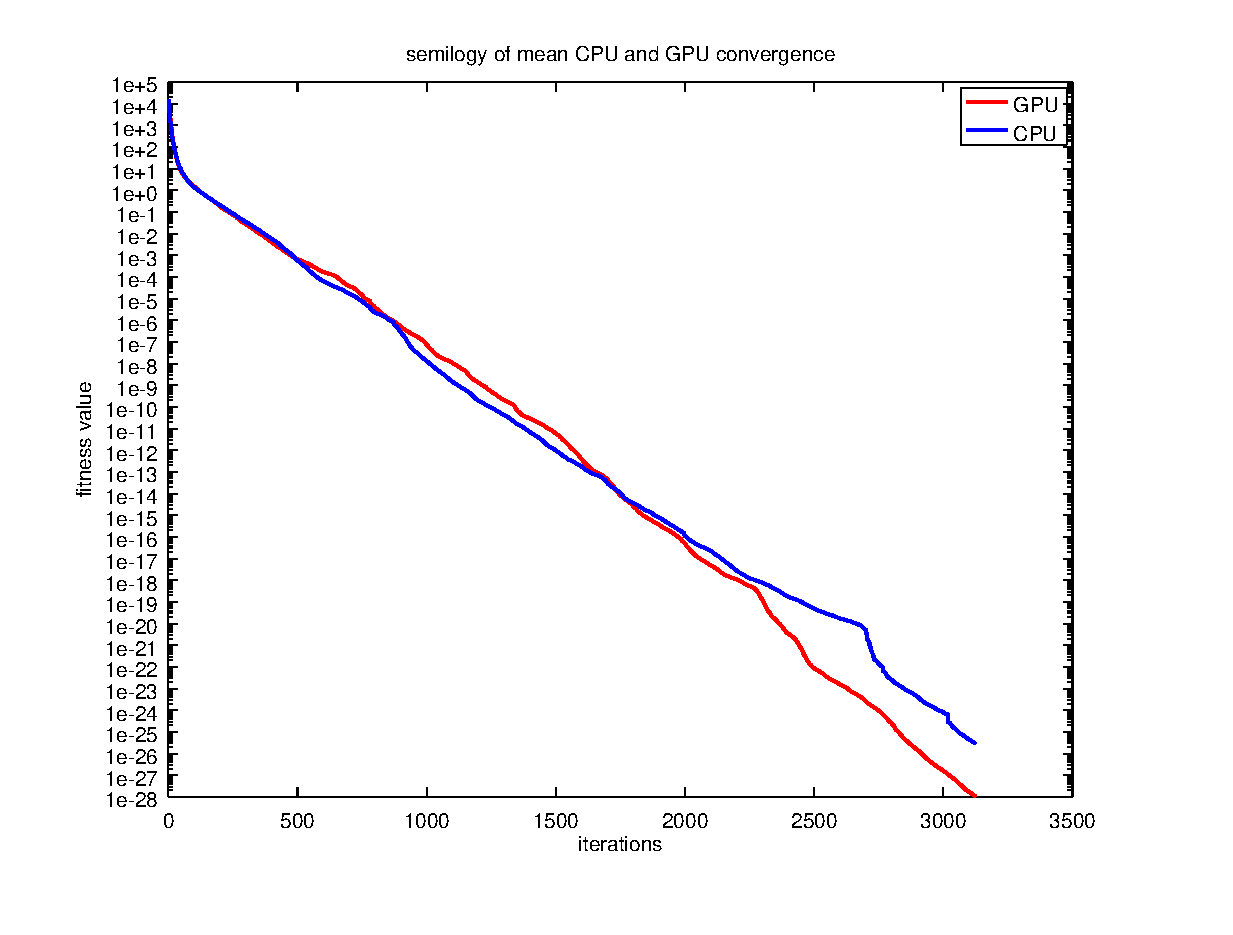
\includegraphics[width=\columnwidth]{../img/semilogy_convergence.eps}
        \caption{semilogy of the average quality of the solutions found by the implemented algorithms during the $3125$ iterations on the Sphere problem with $10$ dimensions. As much more iterations, better is the quality of the solutions. Both CPU and GPU behaves similarly, as they implement the same algorithm. For this experiment the GPU implements $1$ block of $32$ threads and this experiment was repeated $51$ times}
        \label{fig:semilogy_convergence}
    \end{figure}

    Then, we implemented a version using shared memory also.
    The best-known fitness, the previous best, the population (or swarm), the fitness values and the adjacency matrix use shared memory.
    We compare the three versions (CPU, GPU, and GPU with shared memory). In terms of convergence the results were similar (as they should [Figure~\ref{fig:sphere10_32particles_fitness}]).
    That indicates that the GPU implementation using shared memory is equivalent to the previous GPU and CPU version in terms of quality of solutions.
    The experiments were repeated $51$ times with the GPU versions using just one block with $32$ threads. The GPU with shared memory was $1.1377$ times faster in average than GPU without using shared memory. But, the CPU implementation was the fastest: $2.87$ times faster than GPU (Figure~\ref{fig:sphere10_32particles_time}).
    Those results show that the GPU using only one block of $32$ threads is not competitive against the CPU. As the implementation using shared memory was faster than the previous one, it is the default GPU implementation used in the next experiments.


    \begin{figure}[!htb]
        \centering
        \includegraphics[width=\columnwidth]{../img/sphere10_32particles_fitness.eps}
        \caption{Boxplot of the quality of the output solution set generated by the algorithms (CPU, GPU and GPU using shared memory) on the Sphere problem with $10$ dimensions. All implementations behave similarly (in terms of quality of result) as they implement the same algorithm. Both GPU implementations use $1$ block of $32$ threads and this experiment was repeated $51$ times.}
        % \caption{Convergence of different implementations (single block - 51 executions)}
        \label{fig:sphere10_32particles_fitness}
    \end{figure}


    \begin{figure}[!htb]
        \centering
        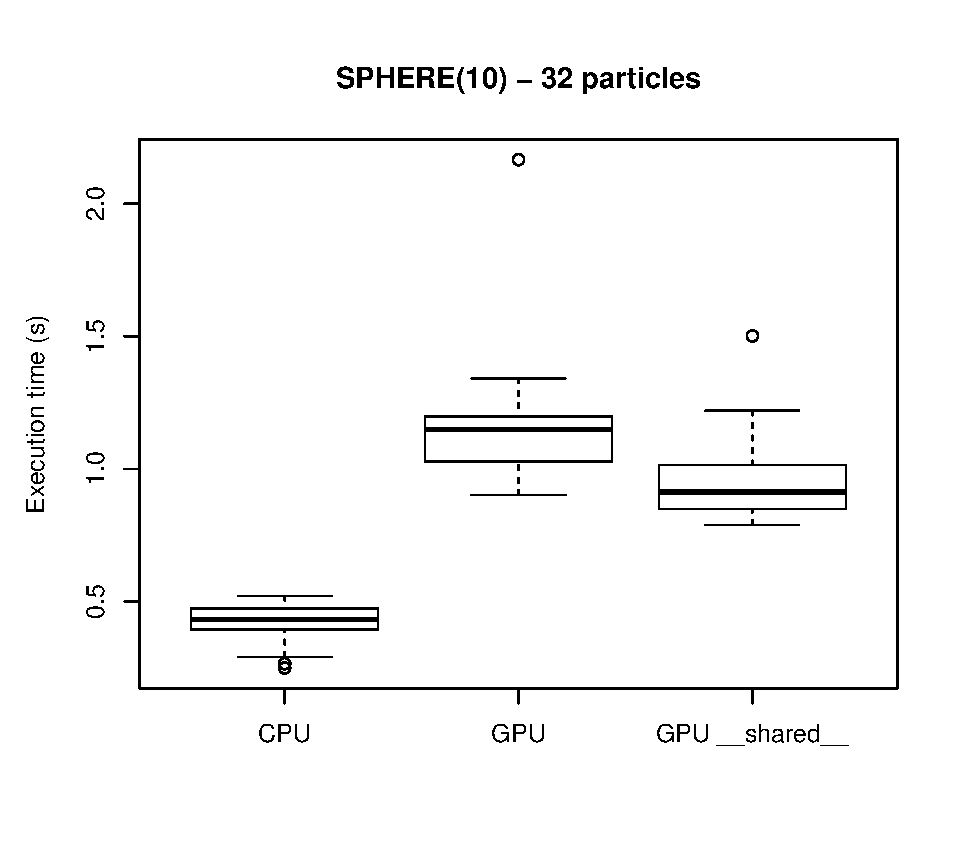
\includegraphics[width=\columnwidth]{../img/sphere10_32particles_time.eps}
        \caption{Boxplot of the exexution time (in seconds) of the implemented algorithms (CPU, GPU and GPU using shared memory) on the Sphere problem with $10$ dimensions. Both GPU implementations use $1$ block of $32$ threads and this experiment was repeated $51$ times. In this experiment the CPU version was about $3$ times faster then GPUs, running in most cases in less than half second. The GPU versions executed generally close to one second, but the version with shared memory ran faster. (Experiments with more threads and blocks are presented further)}
        % \caption{Execution time of different implementations (single block - 51 executions)} 
        \label{fig:sphere10_32particles_time}
    \end{figure}


    \subsection{Multi-blocks experiments}

    To use the CUDA parallelism capabilities and exploit the characteristics of SPSO it was created another GPU code implementation that executes the $51$ runs in parallel using $51$ blocks. To evaluate the execution time we repeat the experiment $30$ times. For comparison, it was also implemented a CPU version that computes the $51$ independent runs but iteratively.
    Again it is first evaluated if the quality of the result is equivalent between the CPU and GPU implementations.
    The fitness of the GPU (with shared memory) and CPU continued to be similar (Figure~\ref{fig:sphere10_32particles_multi_runs_fitness}) but the execution time of the GPU was faster than CPU (Figure~\ref{fig:sphere10_32particles_multi_runs_time}).
    Using $51$ blocks to execute the $51$ independent runs of the algorithm the GPU implementation was $12$ times faster than CPU. The execution of the GPU code took $0.346$ seconds in average. While the CPU code took $12.849$ seconds in average.


    \begin{figure}[!htb]
        \centering
        \includegraphics[width=\columnwidth]{../img/sphere10_32particles_multi_runs_fitness.eps}
        \caption{Boxplot of the quality of the solutions generated by CPU and GPU (with shared memory) versions on the Sphere problem with $10$ dimensions. In this experiment the GPU uses $51$ blocks of $32$ threads and the experiment was repeated $30$ times. The implementations behave similarly (in terms of quality) as they implement the same algorithm.}
        \label{fig:sphere10_32particles_multi_runs_fitness}
    \end{figure}


    \begin{figure}[!htb]
        \centering
        \includegraphics[width=\columnwidth]{../img/sphere10_32particles_multi_runs_time.eps}
        \caption{Boxplot of the execution time (in seconds) of CPU and GPU (with shared memory) on the Sphere problem with $10$ dimensions. In this experiment the GPU uses $51$ blocks of $32$ threads and the experiment was repeated $30$ times. The GPU was $12$ times faster than CPU.}
        % \caption{Execution time of different implementations (GPU 51-blocks, 30 repetitions)}
        \label{fig:sphere10_32particles_multi_runs_time}
    \end{figure}


    \subsection{Scalability experiments}

    To evaluate a better use of the GPU capabilities some experiments were made in order to evaluate:
    \begin{enumerate}
        \item How the implementations behave in a more complicated problem?
        \item It is possible to improve the quality of the solutions, increasing the size of the population (that defines the number of threads)?
        \item How the increasing of the size of the population affects the execution time?
    \end{enumerate}

    For this experiment we use the Schaffer's function~\cite{Schaffer} (presented by Figure~\ref{fig:schaffer}.
    A minimization problem: 

    \begin{equation}
        f(x_0 \cdots x_n) = [\frac{1}{n-1}\sqrt{s_i} \cdot (sin(50.0s_i^{\frac{1}{5}})+1)]^2 s_i = \sqrt{x_i^2 + x_{i+1}^2}
    \end{equation}

    \begin{equation}
            100.0 \leq x_i \leq 100.0
    \end{equation}

    \begin{equation}
        \text{minimum at }f(0, \cdots, 0) = 0
    \end{equation}

     \begin{figure}[!htb]
        \centering
        \includegraphics[width=\columnwidth]{../img/schafferf7.png}
        \caption{Schaffer's F7 --- Two dimensional view}
        % \caption{Execution time of different implementations (GPU 51-blocks, 30 repetitions)}
        \label{fig:schaffer}
    \end{figure}

    The Schaffer problem is far more complex than Sphere and it is also present on the COCO (Comparing Continuous Optimisers) benchmark~\footnote{http://coco.gforge.inria.fr/}.
    In a first experiment, it was checked if the GPU and CPU implementations obtain equivalent results in this new problem. Figure~\ref{fig:schaffer10_32particles_fitness} shows that they did obtain equivalent results in terms of quality of solutions.
    Then it was evaluated the execution time, in this experiment the GPU uses $51$ blocks of $32$ threads and the experiment was repeated $30$ times. The CPU implementation took $19.391$ seconds in average, while the GPU implementation took only $1.154$ seconds in average. So, the GPU was $16.8$ times faster than CPU (Figure~\ref{fig:schaffer10_32particles_time}).

    \begin{figure}[!htb]
        \centering
        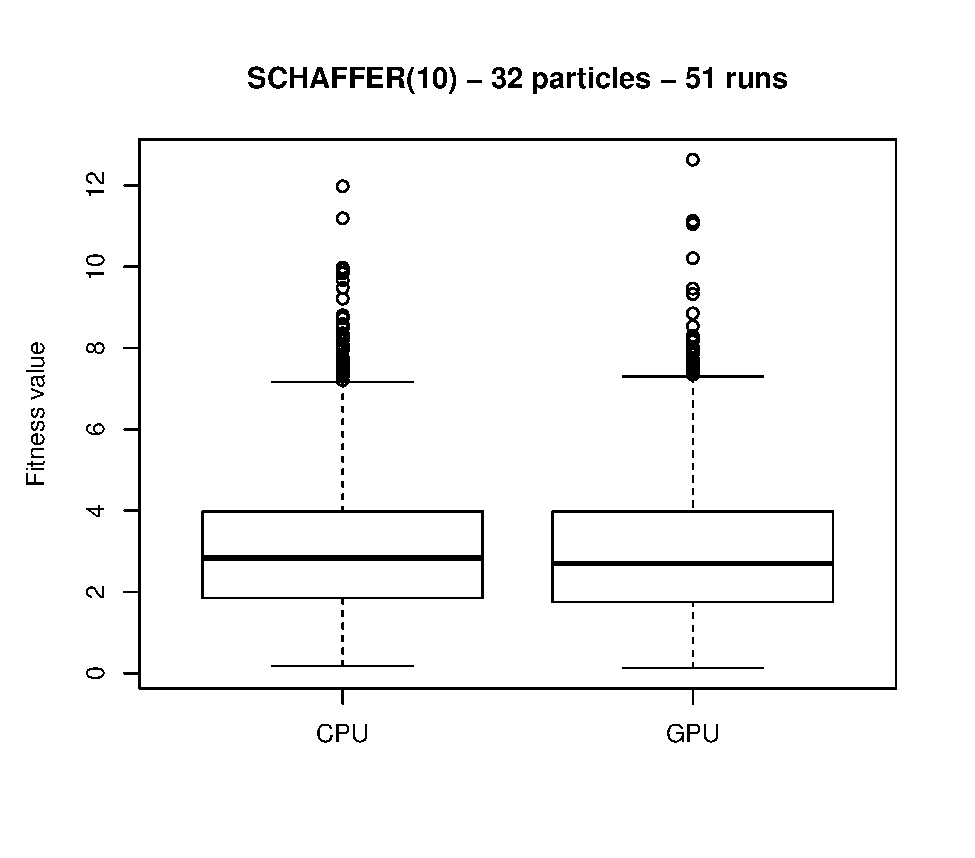
\includegraphics[width=\columnwidth]{../img/schaffer10_32particles_fitness.eps}
        \caption{Boxplot of the quality of the solutions on the problem Schaffer with $10$ dimensions. In this experiment the GPU uses $51$ blocks of $32$ threads and the experiment was repeated $30$ times. The quality of the result is similar as they implement the same algorithm.}
        \label{fig:schaffer10_32particles_fitness}
    \end{figure}

    
    \begin{figure}[!htb]
        \centering
        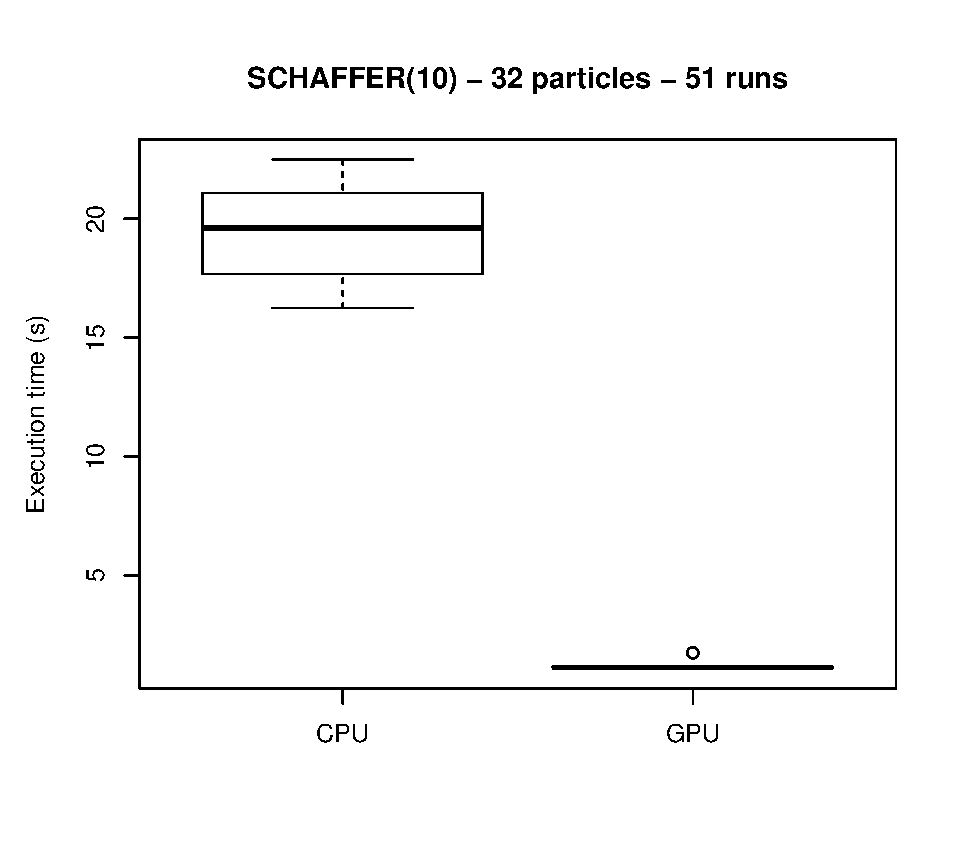
\includegraphics[width=\columnwidth]{../img/schaffer10_32particles_time.eps}
        \caption{Boxplot of the execution time (in seconds) of GPU and CPU versions on the Schaffer problem with $10$ dimensions. In this experiment the GPU uses $51$ blocks of $32$ threads and the experiment was repeated $30$ times. The GPU version was about $16.8$ times faster then CPU.}
        \label{fig:schaffer10_32particles_time}
    \end{figure}

    To evaluate the scalability of the algorithms increasing the population size (and consequently the number of threads) an experiment was performed.
    The population size was set from $32$ up to $160$, increasing $32$ each time ({\it i.e.} \{$32$, $64$, $96$, $128$, $160$\}). The number of threads was not set above $160$ to exploit the use of shared memory. From Figure~\ref{fig:scalability_schafferf7} it is possible to observe that the quality of the solutions improves increasing the population size. Also, both CPU and GPU obtain equivalent results (in terms of quality of output) mainly from $32$ to $64$.

    \begin{figure}[!htb]
        \centering
        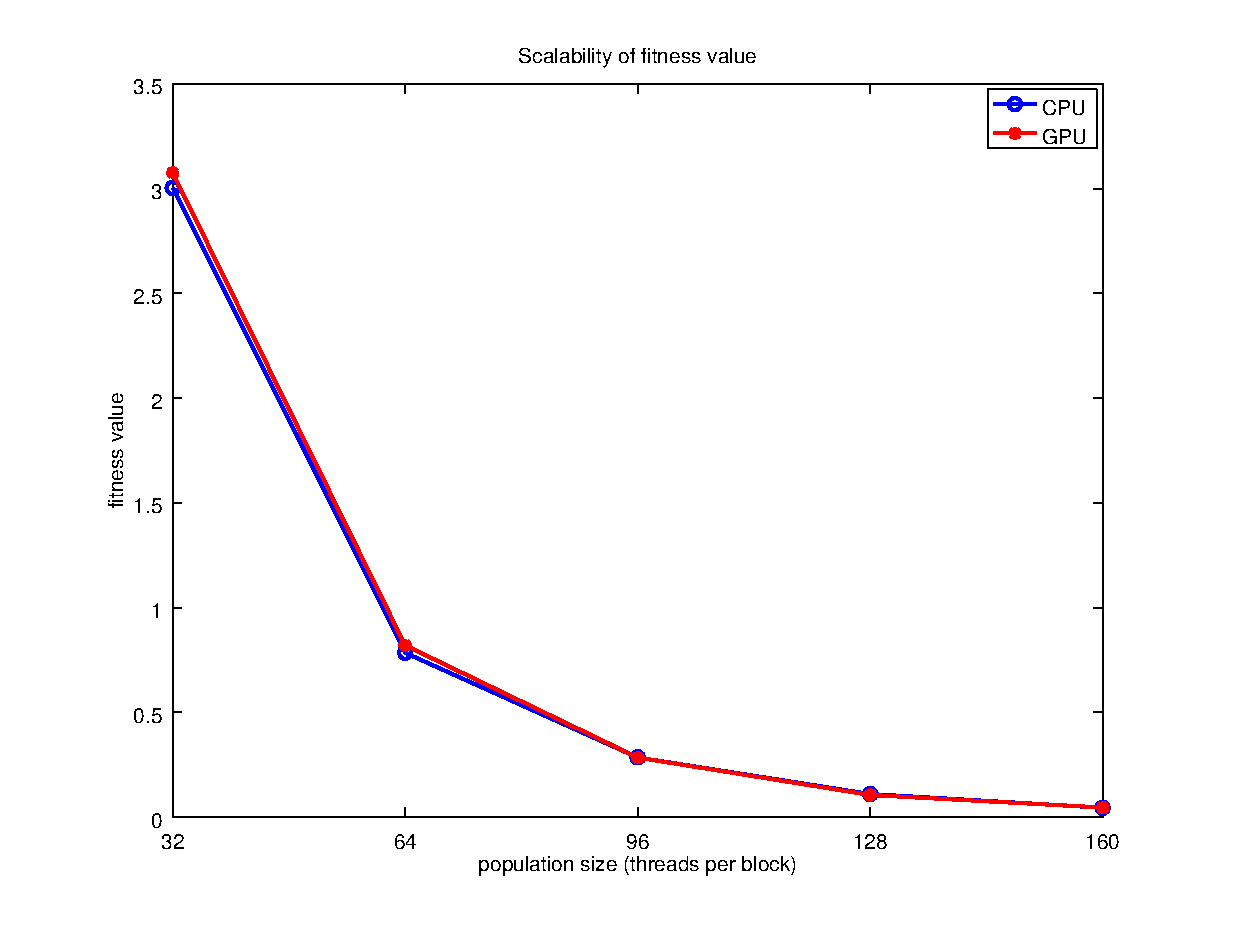
\includegraphics[width=\columnwidth]{../img/scalability_schafferf7.eps}
        \caption{Scalability of the quality: average quality of the implementations (CPU and GPU) when increasing the population size. In this experiment the GPU uses $51$ blocks and the population size defines the number of threads. The experiment was repeated $30$ times. Both algorithms perform similarly, as much more population size, better the quality of the solutions.}
        \label{fig:scalability_schafferf7}
    \end{figure}

    It was also evaluated the scalability in terms of execution time (Figure~\ref{fig:scalability_schafferf7_time}).
    For both GPU and CPU increasing the population size (threads per block) increases the execution time.
    Although, the CPU time increases more drastically. From $32$ to $160$ the CPU execution time increased from $23.8$ seconds to $108.7$ seconds, while the GPU time increased from $1.22$ seconds to $5.45$. The Table~\ref{tbl:scalability} presents the scalability of GPU and CPU increasing the population size. For both GPU and CPU the population size of $32$ is the fastest to execute, $1.2$ seconds to GPU and $23.8$ seconds to CPU ($19.4$ times slower). The best speedup is obtained with $64$ threads per block, $26$ times faster than CPU. For $96$ threads per block, the GPU needed almost $3$ seconds to execute, while the CPU took almost $70$. The smallest speed up was achieved with a population size of $128$, only $16.5$ times faster than CPU. The population size of $160$ is the highest value used, it is the value that uses more the device capabilities (in terms of threads per block and usage of shared memory). In addition, it is the slowest to run, but also is the one with the best quality of solutions. For a population of $160$, the speedup was about $20$ times faster than CPU.

    \begin{figure}[!htb]
        \centering
        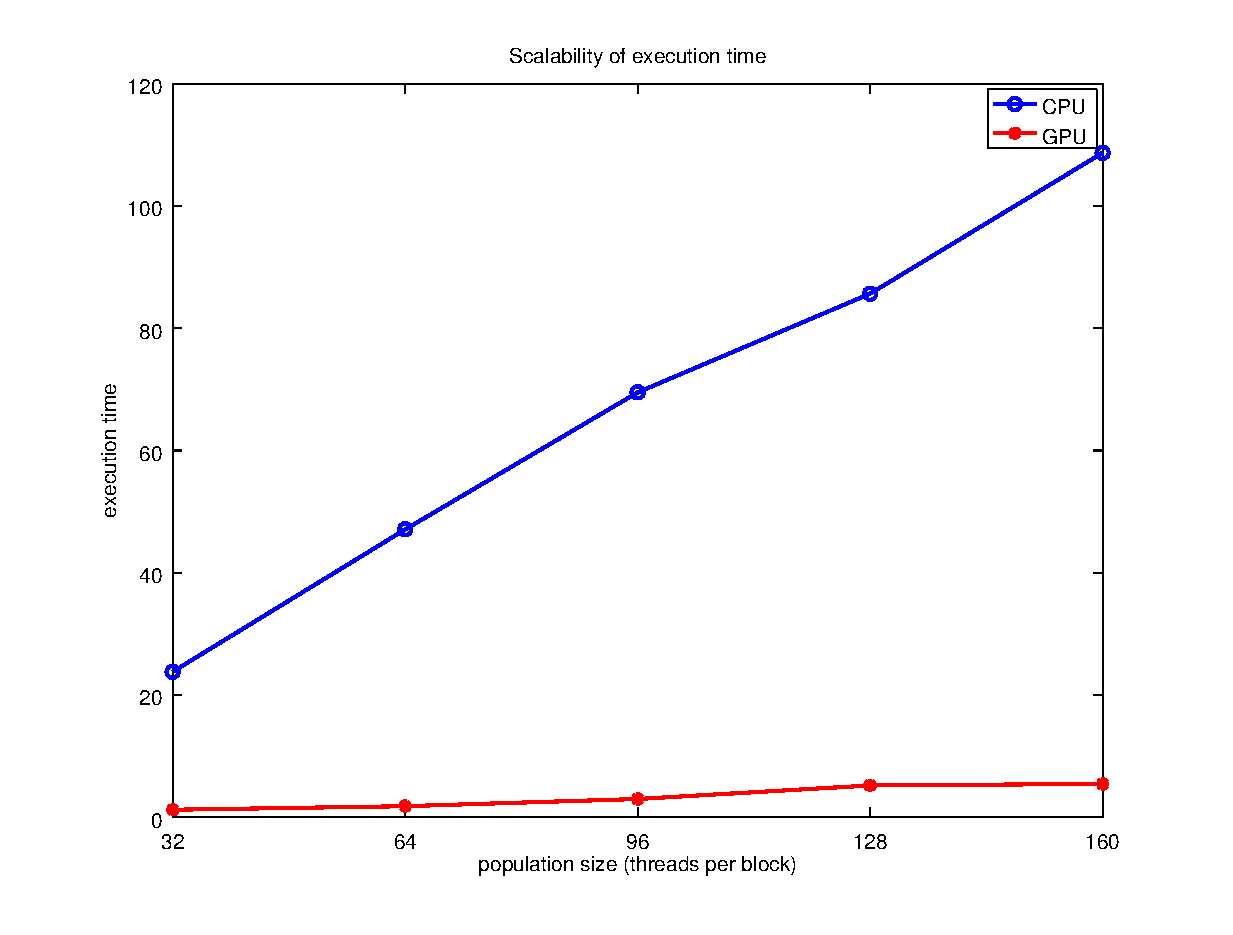
\includegraphics[width=\columnwidth]{../img/scalability_schafferf7_time.eps}
        \caption{Scalability of the execution time (in seconds): average execution time (s) of the implementations (CPU and GPU) when increasing the population size. In this experiment the GPU uses $51$ blocks and the population size defines the number of threads. The experiment was repeated $30$ times. The average GPU speed up was $21$ times faster than CPU. From $32$ to $160$  threads the CPU execution time increased from $23.8$ seconds to $108.7$ seconds, while the GPU time increased from $1.22$ seconds to $5.45$.}
        \label{fig:scalability_schafferf7_time}
    \end{figure}

    \begin{table*}[!t]
        \centering
        \caption{Scalability of GPU and CPU increasing the population size. In this experiment the GPU uses $51$ blocks and the population size defines the number of threads. The experiment was repeated $30$ times. The best speed up was achived using $64$ threads per block while the worst was using $128$ threads per block.}
        \label{tbl:scalability}
        \begin{tabular}{|c|r|r|r|}
        \hline
        \textbf{population (threads per block)} & \multicolumn{1}{c|}{\textbf{GPU time (s)}} & \multicolumn{1}{c|}{\textbf{CPU time (s)}} & \multicolumn{1}{c|}{\textbf{GPU speed up}} \\ \hline
        32                       & 1.2274                                     & 23.8012                                    & 19.3909x                                   \\ \hline
        64                       & 1.8086                                     & 47.0796                                    & 26.0313x                                   \\ \hline
        96                       & 2.9866                                     & 69.5055                                    & 23.2725x                                   \\ \hline
        128                      & 5.2027                                     & 85.6585                                    & 16.4643x                                   \\ \hline
        160                      & 5.4543                                     & 108.7034                                   & 19.9297x                                   \\ \hline
        \end{tabular}
    \end{table*}


    \section{Conclusions}

    In this project, we implement a Parallel Standard Particle Swarm Optimization.
    For this, we use several concepts of CUDA parallel programming, such as the use of shared memory, thread synchronization, and atomic operations.
    We start with simple tests to evaluate and validate the implementations.
    After validate that both CPU and GPU implementations are equivalent, we evaluate the execution time using shared memory and without use it. The version using shared memory was faster than the previous one. After those initial experiments, we start exploiting the capabilities of the CUDA device and also the characteristics of the problem. The SPSO is a stochastic algorithm, due to that it needs to be executed several times to avoid the effect of randomness to the result. With this in mind, instead of creating a code that implements one execution of SPSO in parallel (and run it several times), we created an implementation capable of executing several SPSO at once in parallel (using several independent blocks), each one also parallels inside their blocks. The suggested number of independent runs is $51$~\cite{SPSO}. Using this approach the GPU implementation was about $12$ times faster than CPU for the Sphere problem and $16.8$ times faster for the Schaffer problem.
    Also, it was analyzed the scalability in terms of population size.
    It was found that as higher the population size, better is the quality of the solutions.
    Also, using the proposed approach, it was possible to increase the population size $5$ times.
    The parallel GPU program executed in five and a half seconds while the CPU version executed for almost two minutes ($1'48''7034$). Finally, we conclude that the best configuration and implementation found is the GPU implementation using a population size of $160$, which found the best solutions ($66$ times better than with $32$) in just a few seconds ($0'05''4543$).



    \bibliographystyle{plain}
    \bibliography{bibliography} 

\end{document}
